\chapter{The Insult}

At the banker’s door Beauchamp stopped Morcerf.

“Listen,” said he; “just now I told you it was of M. de Monte Cristo
you must demand an explanation.”

“Yes; and we are going to his house.”

“Reflect, Morcerf, one moment before you go.”

“On what shall I reflect?”

“On the importance of the step you are taking.”

“Is it more serious than going to M. Danglars?”

“Yes; M. Danglars is a money-lover, and those who love money, you know,
think too much of what they risk to be easily induced to fight a duel.
The other is, on the contrary, to all appearance a true nobleman; but
do you not fear to find him a bully?”

“I only fear one thing; namely, to find a man who will not fight.”

“Do not be alarmed,” said Beauchamp; “he will meet you. My only fear is
that he will be too strong for you.”

“My friend,” said Morcerf, with a sweet smile, “that is what I wish.
The happiest thing that could occur to me, would be to die in my
father’s stead; that would save us all.”

“Your mother would die of grief.”

“My poor mother!” said Albert, passing his hand across his eyes, “I
know she would; but better so than die of shame.”

“Are you quite decided, Albert?”

“Yes; let us go.”

“But do you think we shall find the count at home?”

“He intended returning some hours after me, and doubtless he is now at
home.”

They ordered the driver to take them to No. 30 Champs-Élysées.
Beauchamp wished to go in alone, but Albert observed that as this was
an unusual circumstance he might be allowed to deviate from the usual
etiquette of duels. The cause which the young man espoused was one so
sacred that Beauchamp had only to comply with all his wishes; he
yielded and contented himself with following Morcerf. Albert sprang
from the porter’s lodge to the steps. He was received by Baptistin. The
count had, indeed, just arrived, but he was in his bath, and had
forbidden that anyone should be admitted.

“But after his bath?” asked Morcerf.

“My master will go to dinner.”

“And after dinner?”

“He will sleep an hour.”

“Then?”

“He is going to the Opera.”

“Are you sure of it?” asked Albert.

“Quite, sir; my master has ordered his horses at eight o’clock
precisely.”

“Very good,” replied Albert; “that is all I wished to know.”

Then, turning towards Beauchamp, “If you have anything to attend to,
Beauchamp, do it directly; if you have any appointment for this
evening, defer it till tomorrow. I depend on you to accompany me to the
Opera; and if you can, bring Château-Renaud with you.”

Beauchamp availed himself of Albert’s permission, and left him,
promising to call for him at a quarter before eight. On his return
home, Albert expressed his wish to Franz Debray, and Morrel, to see
them at the Opera that evening. Then he went to see his mother, who
since the events of the day before had refused to see anyone, and had
kept her room. He found her in bed, overwhelmed with grief at this
public humiliation.

The sight of Albert produced the effect which might naturally be
expected on Mercédès; she pressed her son’s hand and sobbed aloud, but
her tears relieved her. Albert stood one moment speechless by the side
of his mother’s bed. It was evident from his pale face and knit brows
that his resolution to revenge himself was growing weaker.

“My dear mother,” said he, “do you know if M. de Morcerf has any
enemy?”

Mercédès started; she noticed that the young man did not say “my
father.”

“My son,” she said, “persons in the count’s situation have many secret
enemies. Those who are known are not the most dangerous.”

“I know it, and appeal to your penetration. You are of so superior a
mind, nothing escapes you.”

“Why do you say so?”

“Because, for instance, you noticed on the evening of the ball we gave,
that M. de Monte Cristo would eat nothing in our house.”

Mercédès raised herself on her feverish arm.

“M. de Monte Cristo!” she exclaimed; “and how is he connected with the
question you asked me?”

\begin{figure}[ht]
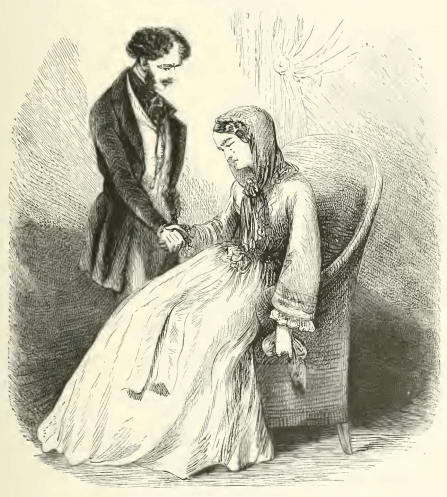
\includegraphics[width=\textwidth]{40219m.jpg}
\end{figure}

“You know, mother, M. de Monte Cristo is almost an Oriental, and it is
customary with the Orientals to secure full liberty for revenge by not
eating or drinking in the houses of their enemies.”

“Do you say M. de Monte Cristo is our enemy?” replied Mercédès,
becoming paler than the sheet which covered her. “Who told you so? Why,
you are mad, Albert! M. de Monte Cristo has only shown us kindness. M.
de Monte Cristo saved your life; you yourself presented him to us. Oh,
I entreat you, my son, if you had entertained such an idea, dispel it;
and my counsel to you—nay, my prayer—is to retain his friendship.”

“Mother,” replied the young man, “you have special reasons for telling
me to conciliate that man.”

“I?” said Mercédès, blushing as rapidly as she had turned pale, and
again becoming paler than ever.

“Yes, doubtless; and is it not that he may never do us any harm?”

Mercédès shuddered, and, fixing on her son a scrutinizing gaze, “You
speak strangely,” said she to Albert, “and you appear to have some
singular prejudices. What has the count done? Three days since you were
with him in Normandy; only three days since we looked on him as our
best friend.”

An ironical smile passed over Albert’s lips. Mercédès saw it and with
the double instinct of woman and mother guessed all; but as she was
prudent and strong-minded she concealed both her sorrows and her fears.
Albert was silent; an instant after, the countess resumed:

“You came to inquire after my health; I will candidly acknowledge that
I am not well. You should install yourself here, and cheer my solitude.
I do not wish to be left alone.”

“Mother,” said the young man, “you know how gladly I would obey your
wish, but an urgent and important affair obliges me to leave you for
the whole evening.”

“Well,” replied Mercédès, sighing, “go, Albert; I will not make you a
slave to your filial piety.”

Albert pretended he did not hear, bowed to his mother, and quitted her.
Scarcely had he shut her door, when Mercédès called a confidential
servant, and ordered him to follow Albert wherever he should go that
evening, and to come and tell her immediately what he observed. Then
she rang for her lady’s maid, and, weak as she was, she dressed, in
order to be ready for whatever might happen. The footman’s mission was
an easy one. Albert went to his room, and dressed with unusual care. At
ten minutes to eight Beauchamp arrived; he had seen Château-Renaud, who
had promised to be in the orchestra before the curtain was raised. Both
got into Albert’s \textit{coupé}; and, as the young man had no reason to
conceal where he was going, he called aloud, “To the Opera.” In his
impatience he arrived before the beginning of the performance.

\begin{figure}[ht]
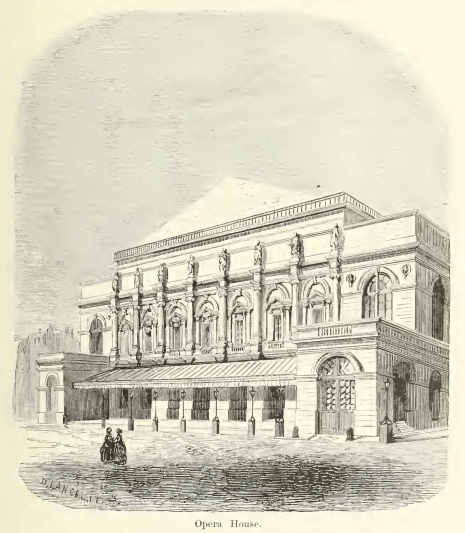
\includegraphics[width=\textwidth]{40221m.jpg}
\end{figure}

Château-Renaud was at his post; apprised by Beauchamp of the
circumstances, he required no explanation from Albert. The conduct of
the son in seeking to avenge his father was so natural that
Château-Renaud did not seek to dissuade him, and was content with
renewing his assurances of devotion. Debray was not yet come, but
Albert knew that he seldom lost a scene at the Opera.

Albert wandered about the theatre until the curtain was drawn up. He
hoped to meet with M. de Monte Cristo either in the lobby or on the
stairs. The bell summoned him to his seat, and he entered the orchestra
with Château-Renaud and Beauchamp. But his eyes scarcely quitted the
box between the columns, which remained obstinately closed during the
whole of the first act. At last, as Albert was looking at his watch for
about the hundredth time, at the beginning of the second act the door
opened, and Monte Cristo entered, dressed in black, and, leaning over
the front of the box, looked around the pit. Morrel followed him, and
looked also for his sister and brother in-law; he soon discovered them
in another box, and kissed his hand to them.

The count, in his survey of the pit, encountered a pale face and
threatening eyes, which evidently sought to gain his attention. He
recognized Albert, but thought it better not to notice him, as he
looked so angry and discomposed. Without communicating his thoughts to
his companion, he sat down, drew out his opera-glass, and looked
another way. Although apparently not noticing Albert, he did not,
however, lose sight of him, and when the curtain fell at the end of the
second act, he saw him leave the orchestra with his two friends. Then
his head was seen passing at the back of the boxes, and the count knew
that the approaching storm was intended to fall on him. He was at the
moment conversing cheerfully with Morrel, but he was well prepared for
what might happen.

The door opened, and Monte Cristo, turning round, saw Albert, pale and
trembling, followed by Beauchamp and Château-Renaud.

“Well,” cried he, with that benevolent politeness which distinguished
his salutation from the common civilities of the world, “my cavalier
has attained his object. Good-evening, M. de Morcerf.”

The countenance of this man, who possessed such extraordinary control
over his feelings, expressed the most perfect cordiality. Morrel only
then recollected the letter he had received from the viscount, in
which, without assigning any reason, he begged him to go to the Opera,
but he understood that something terrible was brooding.

“We are not come here, sir, to exchange hypocritical expressions of
politeness, or false professions of friendship,” said Albert, “but to
demand an explanation.”

The young man’s trembling voice was scarcely audible.

“An explanation at the Opera?” said the count, with that calm tone and
penetrating eye which characterize the man who knows his cause is good.
“Little acquainted as I am with the habits of Parisians, I should not
have thought this the place for such a demand.”

“Still, if people will shut themselves up,” said Albert, “and cannot be
seen because they are bathing, dining, or asleep, we must avail
ourselves of the opportunity whenever they are to be seen.”

“I am not difficult of access, sir; for yesterday, if my memory does
not deceive me, you were at my house.”

“Yesterday I was at your house, sir,” said the young man; “because then
I knew not who you were.”

In pronouncing these words Albert had raised his voice so as to be
heard by those in the adjoining boxes and in the lobby. Thus the
attention of many was attracted by this altercation.

“Where are you come from, sir? “ said Monte Cristo “You do not appear
to be in the possession of your senses.”

“Provided I understand your perfidy, sir, and succeed in making you
understand that I will be revenged, I shall be reasonable enough,” said
Albert furiously.

“I do not understand you, sir,” replied Monte Cristo; “and if I did,
your tone is too high. I am at home here, and I alone have a right to
raise my voice above another’s. Leave the box, sir!”

Monte Cristo pointed towards the door with the most commanding dignity.

“Ah, I shall know how to make you leave your home!” replied Albert,
clasping in his convulsed grasp the glove, which Monte Cristo did not
lose sight of.

“Well, well,” said Monte Cristo quietly, “I see you wish to quarrel
with me; but I would give you one piece of advice, which you will do
well to keep in mind. It is in poor taste to make a display of a
challenge. Display is not becoming to everyone, M. de Morcerf.”

At this name a murmur of astonishment passed around the group of
spectators of this scene. They had talked of no one but Morcerf the
whole day. Albert understood the allusion in a moment, and was about to
throw his glove at the count, when Morrel seized his hand, while
Beauchamp and Château-Renaud, fearing the scene would surpass the
limits of a challenge, held him back. But Monte Cristo, without rising,
and leaning forward in his chair, merely stretched out his arm and,
taking the damp, crushed glove from the clenched hand of the young man:

“Sir,” said he in a solemn tone, “I consider your glove thrown, and
will return it to you wrapped around a bullet. Now leave me or I will
summon my servants to throw you out at the door.”

Wild, almost unconscious, and with eyes inflamed, Albert stepped back,
and Morrel closed the door. Monte Cristo took up his glass again as if
nothing had happened; his face was like marble, and his heart was like
bronze. Morrel whispered, “What have you done to him?”

“I? Nothing—at least personally,” said Monte Cristo.

“But there must be some cause for this strange scene.”

“The Count of Morcerf’s adventure exasperates the young man.”

“Have you anything to do with it?”

“It was through Haydée that the Chamber was informed of his father’s
treason.”

“Indeed?” said Morrel. “I had been told, but would not credit it, that
the Grecian slave I have seen with you here in this very box was the
daughter of Ali Pasha.”

“It is true, nevertheless.”

“Then,” said Morrel, “I understand it all, and this scene was
premeditated.”

“How so?”

“Yes. Albert wrote to request me to come to the Opera, doubtless that I
might be a witness to the insult he meant to offer you.”

“Probably,” said Monte Cristo with his imperturbable tranquillity.

“But what shall you do with him?”

“With whom?”

“With Albert.”

“What shall I do with Albert? As certainly, Maximilian, as I now press
your hand, I shall kill him before ten o’clock tomorrow morning.”
Morrel, in his turn, took Monte Cristo’s hand in both of his, and he
shuddered to feel how cold and steady it was.

“Ah, count,” said he, “his father loves him so much!”

“Do not speak to me of that,” said Monte Cristo, with the first
movement of anger he had betrayed; “I will make him suffer.”

Morrel, amazed, let fall Monte Cristo’s hand. “Count, count!” said he.

“Dear Maximilian,” interrupted the count, “listen how adorably Duprez
is singing that line,—

\begin{quote}
{\small‘O Mathilde! idole de mon âme!’}
\end{quote}

“I was the first to discover Duprez at Naples, and the first to applaud
him. Bravo, bravo!”

Morrel saw it was useless to say more, and refrained. The curtain,
which had risen at the close of the scene with Albert, again fell, and
a rap was heard at the door.

“Come in,” said Monte Cristo with a voice that betrayed not the least
emotion; and immediately Beauchamp appeared. “Good-evening, M.
Beauchamp,” said Monte Cristo, as if this was the first time he had
seen the journalist that evening; “be seated.”

Beauchamp bowed, and, sitting down, “Sir,” said he, “I just now
accompanied M. de Morcerf, as you saw.”

“And that means,” replied Monte Cristo, laughing, “that you had,
probably, just dined together. I am happy to see, M. Beauchamp, that
you are more sober than he was.”

“Sir,” said M. Beauchamp, “Albert was wrong, I acknowledge, to betray
so much anger, and I come, on my own account, to apologize for him. And
having done so, entirely on my own account, be it understood, I would
add that I believe you too gentlemanly to refuse giving him some
explanation concerning your connection with Yanina. Then I will add two
words about the young Greek girl.”

Monte Cristo motioned him to be silent. “Come,” said he, laughing,
“there are all my hopes about to be destroyed.”

“How so?” asked Beauchamp.

“Doubtless you wish to make me appear a very eccentric character. I am,
in your opinion, a Lara, a Manfred, a Lord Ruthven; then, just as I am
arriving at the climax, you defeat your own end, and seek to make an
ordinary man of me. You bring me down to your own level, and demand
explanations! Indeed, M. Beauchamp, it is quite laughable.”

“Yet,” replied Beauchamp haughtily, “there are occasions when probity
commands——”

“M. Beauchamp,” interposed this strange man, “the Count of Monte Cristo
bows to none but the Count of Monte Cristo himself. Say no more, I
entreat you. I do what I please, M. Beauchamp, and it is always well
done.”

“Sir,” replied the young man, “honest men are not to be paid with such
coin. I require honorable guaranties.”

“I am, sir, a living guaranty,” replied Monte Cristo, motionless, but
with a threatening look; “we have both blood in our veins which we wish
to shed—that is our mutual guaranty. Tell the viscount so, and that
tomorrow, before ten o’clock, I shall see what color his is.”

“Then I have only to make arrangements for the duel,” said Beauchamp.

“It is quite immaterial to me,” said Monte Cristo, “and it was very
unnecessary to disturb me at the Opera for such a trifle. In France
people fight with the sword or pistol, in the colonies with the
carbine, in Arabia with the dagger. Tell your client that, although I
am the insulted party, in order to carry out my eccentricity, I leave
him the choice of arms, and will accept without discussion, without
dispute, anything, even combat by drawing lots, which is always stupid,
but with me different from other people, as I am sure to gain.”

“Sure to gain!” repeated Beauchamp, looking with amazement at the
count.

“Certainly,” said Monte Cristo, slightly shrugging his shoulders;
“otherwise I would not fight with M. de Morcerf. I shall kill him—I
cannot help it. Only by a single line this evening at my house let me
know the arms and the hour; I do not like to be kept waiting.”

“Pistols, then, at eight o’clock, in the Bois de Vincennes,” said
Beauchamp, quite disconcerted, not knowing if he was dealing with an
arrogant braggadocio or a supernatural being.

“Very well, sir,” said Monte Cristo. “Now all that is settled, do let
me see the performance, and tell your friend Albert not to come any
more this evening; he will hurt himself with all his ill-chosen
barbarisms: let him go home and go to sleep.”

Beauchamp left the box, perfectly amazed.

“Now,” said Monte Cristo, turning towards Morrel, “I may depend upon
you, may I not?”

“Certainly,” said Morrel, “I am at your service, count; still——”

“What?”

“It is desirable I should know the real cause.”

“That is to say, you would rather not?”

“No.”

“The young man himself is acting blindfolded, and knows not the true
cause, which is known only to God and to me; but I give you my word,
Morrel, that God, who does know it, will be on our side.”

“Enough,” said Morrel; “who is your second witness?”

“I know no one in Paris, Morrel, on whom I could confer that honor
besides you and your brother Emmanuel. Do you think Emmanuel would
oblige me?”

“I will answer for him, count.”

“Well? that is all I require. Tomorrow morning, at seven o’clock, you
will be with me, will you not?”

“We will.”

“Hush, the curtain is rising. Listen! I never lose a note of this opera
if I can avoid it; the music of \textit{William Tell} is so sweet.”
